\documentclass{article}
\usepackage[utf8]{inputenc}
\usepackage{t1enc}
\usepackage[magyar]{babel}
\usepackage{geometry}
\geometry{
 a4paper,
 total={210mm,297mm},
 left=15mm,
 right=15mm,
 top=25mm,
 bottom=15mm,
}            

\usepackage{amsmath}
\usepackage{amssymb}
\frenchspacing

\usepackage{enumitem}
\usepackage{multicol}
\usepackage{calc}
\usepackage{pgf,tikz}
\usetikzlibrary{arrows}
\usetikzlibrary{turtle}
\usetikzlibrary{graphs}
\usetikzlibrary{patterns,snakes}
\usepackage{url}
\usepackage[framemethod=default]{mdframed}

\usepackage{tcolorbox}
\usepackage{minted}


\newcommand{\degre}{\ensuremath{^\circ}}
\newcommand{\tg}{\mathop{\mathrm{tg}}\nolimits}
\newcommand{\ctg}{\mathop{\mathrm{ctg}}\nolimits}
\newcommand{\arc}{\mathop{\mathrm{arc}}\nolimits}
\renewcommand{\arcsin}{\arc\sin}
\renewcommand{\arccos}{\arc\cos}
\newcommand{\arctg}{\arc\tg}
\newcommand{\arcctg}{\arc\ctg}
\newcommand{\forras}[1]{\hfill\textit{(#1)}}

\parskip 8pt
\parindent 0pt

\pagestyle{empty}


\title{Képpont árnyalók és előjeles távolság függvények}

\begin{document}
\maketitle

\section{Képpont árnyalók}

\begin{tcolorbox}[title=Képpont árnyalók]
A \emph{képpont árnyalók} (pixel shaders) olyan programok, amelyeket a számítógépi grafikában használnak.
Léteznek szabványos \emph{árnyaló nyelvek} (például az OpenGL specifikáció részét képező GLSL ES),
amelyeket a grafikus kártyák
is tudnak értelmezni és futtatni. A futtató hardver vagy szoftver egy téglalap alakú tartomány
minden $(x,y)$ pontjára meghívja a képpont árnyaló programot, aminek egy színt kell visszaadnia,
az $(x,y)$ képpont színét.

A színeket általában RGBA kódolással definiáljuk, vagyis $(r, g, b, a)$ alakú négydimenziós
valós vektorokkal írjuk le, ahol $r$, $g$ és $b$ a vörös, zöld és kék komponens 0 és 1 közé eső
értéke, $a$ pedig az átlátszatlanság.

$$\mathcal{S}: \mathbb{R}^2 \mapsto \mathbb{R}^4$$
$$\mathcal{S}(x, y) = (r, g, b, a)$$
\end{tcolorbox}

A képpont árnyaló programok egyik hasznos jellemzője, hogy a készülő kép minden képpontját
egymástól függetlenül színezik ki. Ez jelentősen tudja javítani például számítógépes animációk
sebességét (a másodpercenként kirajzolható képkockák számát), ha a grafikus hardver támogatja
a képpont árnyaló program \emph{párhuzamosított} futtatását.

\subsection{GLSL ES, ShaderToy, Twigl}

Az egyik népszerű online alkalmazás képpont árnyékolók tanulásához az Inigo Quilez által fejlesztett
\url{shadertoy.com}. A következőkben a ShaderToy által használt képpont árnyaló nyelvet fogjuk használni,
ami a GLSL ES egy változata.

\subsubsection{Hello, ShaderToy!}

Az árnyaló nyelv hasonlít a C programozási nyelvhez (ha ez segít valakinek). Az $\mathcal{S}(x,y)$
függvényt a \texttt{mainImage} függvény valósítja meg. A bemenő képpont (pixel) $x$ és $y$ koordinátája
a bemenő \texttt{fragCoord} objektumból olvasható ki: \texttt{fragCoord.x} és \texttt{fragCoord.y}.
A kimenő szín-vektort a \texttt{fragColor} változóban kell kiszámolni.

\glslexample{Példa: ferde négyzetet rajzoló árnyaló}{../00_intro/examples/00hello.glsl}

A fenti példa először normalizájla az input koordinátákat, mielőtt a tényleges árnyaló logikát megvalósítaná.
A 3. sorban a globálisan elérhető \texttt{iResolution} objektum (vektor) felhasználásával eltolja a $(0, 0)$ pontot
a kép középpontjába, majd mindent leoszt az $y$ irányú felbontással. A kapott $y$ érték $-1$ és $1$ közé esik.
(Itt láthatjuk, hogy a legtöbb művelet az árnyaló nyelvekben ,,vektorizált'', a műveletek értik, hogy amikor
vektorokkal dolgoznak, koordinátánként kell-e elvégezni a számolást.)

A 4. sorban feketére vagy fehérre színezzük az $(x, y)$ képpontot attól függöen, hogy teljesül-e
az $|x|+|y| < 0.2$ egyenlőtlenség.
(A fekete szín RGB kódolása három nulla, a \texttt{vec3} \emph{konstruktor}
érti, hogy ha egy paramétert kapott, akkor mindhárom koordinátát arra állítja be.)
A \texttt{vec3(0.9)} világos-szürke hátteret definiál.

Végül az 5. sorban az látható, hogy a ShaderToy aktuális verziójában az $a$ értéke mindig 1.0, vagyis
nem változtatható az átlátszatlanság.


\includegraphics[width=5cm]{images/hello.png}


\subsubsection{GLSL ES}

A GLSL ES nyelv leírása meghaladja ezen jegyzet kereteit.
A nyelv egy rövid kivonata a mellékelt \href{run:./glsl.pdf}{GLSL gyorstalpaló}
dokumentumban olvasható.



\subsubsection{Hello, Twigl!}

Az online ShaderToy egy alternativája a Twigl, amit saját gépünkre telepíthetünk és offline futtathatunk.
A Twigl picit más elnevezéseket használ, ez az alább látható.

\glslexample{Ferde négyzetet rajzoló árnyaló (Twigl verzió)}{../00_intro/examples/00hello_twigl.glsl}
  
A folytatásban a ShaderToy nyelvjárását fogjuk használni. 

\matfeladatok

Első próbálkozásnak kísérletezhetünk különböző színátmenetekkel. Ehhez normalizáljuk 0 és 1 közé
az $x$ koordinátát, majd a képpontok színét adjuk meg ennek függvényeként.

\begin{glsl}{Átmenetek}
float f(float x) { return /*???*/ }
    
void mainImage( out vec4 fragColor, in vec2 fragCoord )
{
  vec2 uv = fragCoord/iResolution.xy;
  vec3 col = vec3(f(uv.x));
  fragColor = vec4(col,1.0);
}
\end{glsl}

Keressünk $f: [0, 1] \mapsto [0,1]$ átmenet függvényeket a következő tulajdonságokkal.
Lehetőleg ne használjunk elágazást (\texttt{if}) csak aritmetikát és függvényeket.

\begin{enumerate}
  \item $f$ lineáris, $f(0)=0$, $f(1)=1$.
  \item $f$ majdnem mindig 0, kivéve amikor $|x-0.5|$ ,,kicsi''.
  \item $f$ majdnem mindig 0, kivéve amikor $x$ ,,közel'' esik $0.1$ valamelyik egész többszöröséhez.
  \item $f$ ,,simán'' köti össze a $(0,0)$ és $(1,1)$ pontokat, a végpontokban vízszintes az érintője.
  \item Ugyanaz, mint előbb, de $f$-ről azt is megköveteljük, hogy polinomfüggvény legyen. 
\end{enumerate}

A fentebb készített ábrákra tegyük rá az $y=f(x)$ függvény grafikonját is.

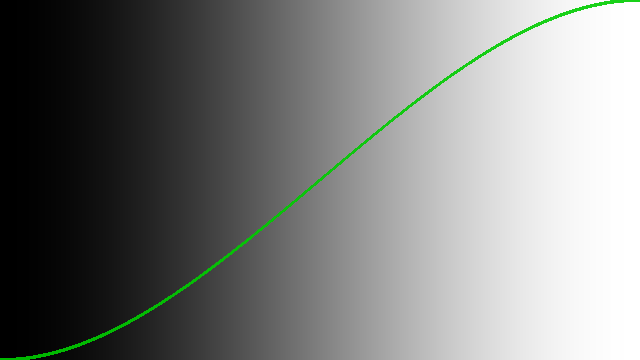
\includegraphics[width=5cm]{images/fv.png}


\subsection{Elemi alakzatok}

A legegyszerűbb ,,modellezési'' megközelítés árnyalókkal az, hogy minden bemeneti koordinátára
eldöntjük, az alakzathoz tartozik-e vagy nem (igen / nem), majd ez alapján vagy az
alakzat színét adjuk vissza, vagy a háttér színét.

\begin{tcolorbox}
  
  $$
  \mathcal{S}: \mathbb{R}^2 \mapsto \mathbb{R}^4,\quad
  \mathcal{A}: \mathbb{R}^2 \mapsto \{igaz, hamis\},\quad
  \mathcal{C}: \{igaz, hamis\} \mapsto \mathbb{R}^4
  $$
  $$\mathcal{S}(x, y) = \mathcal{C}(\mathcal{A}(x,y))$$

  $$\mathcal{A}(x,y) = 
    \begin{cases}
      igaz,  &\text{ha~} (x, y) \text{~az alakzat pontja}\cr
      hamis, &\text{különben}
    \end{cases}
  $$

  $$\mathcal{C}(l) = 
    \begin{cases}
      \text{alakzat szín},  &\text{ha~} l\cr
      \text{háttér szín}, &\text{különben}
    \end{cases}
  $$

  \end{tcolorbox}

\progfeladatok

\begin{enumerate}
  \item Rajzoljunk adott sugarú kört origó középponttal.
  \item Rajzoljunk adott méretű négyzetet origó középponttal.
  \item Rajzoljunk adott méretű téglalapot adott középponttal.
  \item Rajzoljunk négyzetrácsot.
  \item Színezzük ki a képet sakktábla-szerűen.
  \item (*) Rajzoljunk szabályos háromszöget.
  \item (*) Rajzoljunk szabályos sokszöget.
\end{enumerate}

\subsection{Polár-koordináták}

Az \texttt{atan} függvény segítségével egyszerűen átalakíthatunk egy Descartes-koordinátákkal adott
pontot polárkoordinátás alakba:

\begin{glsl}{Polárkoordináták}
float r = length(p);
float alpha = atan(p.y, p.x);
\end{glsl}

Az \texttt{atan} függvény $-\pi$ és $\pi$ közé eső értéket ad, a 0 az X tengely pozitív irányának felel meg.
Szürke árnyalatokkal illusztrálva ($-\pi$ a fekete, $\pi$ a fehér árnyalat):


\includegraphics[width=5cm]{images/atan.png}

\progfeladatok

\begin{enumerate}
  \item Rajzoljunk ,,napot'' adott számú ,,napsugárral''.
  \item Rajzoljunk szabályos háromszöget, mint ,,változó sugarú kört''.
\end{enumerate}

\subsection{Transzformációk és animáció}

\subsubsection{Geometriai transzformációk}

Egy $g$ síkbeli geometriai transzformáció a sík minden pontjához a sík valamelyik pontját rendeli.

$$g(x, y) = (x', y')$$

\matfeladatok

\begin{enumerate}
  \item Adott egy síkbeli $\mathcal{A}$ alakzat az $\mathcal{S}()$ árnyalóval leírva. Hogyan állítható elő
  az $\mathcal{A}' = g(\mathcal{A})$ alakzat árnyalója?
  \item Adjuk meg a következő transzformációkat formulával:
  (a) eltolás adott vektorral;
  (b) origó körüli forgatás;
  (c) origó középpontú nagyítás;
  (d) origó középpontú, egységsugarú inverzió.
\end{enumerate}

\subsubsection{Animációk}
Az árnyékolók nagyon egyszerűen használhatók animációk programozására, csupán
be kell vezetnünk egy idő input változót:

$$\mathcal{S}(x, y, t) = (r, g, b, a)$$

A Shadertoy esetében ez az input változó az \texttt{iTime}, ami másodpercben méri az animáció indítása
óta eltelt időt. Egy képkocka kiszámítása közben minden árnyaló hívás azonos $t$ értéket kap.

Az alábbi példában a kirajzolt kör középpontja
az eltelt időtől függően változik.

\glslexample{,,Pattogó'' labda}{../00_intro/examples/90bouncingb.glsl}

\progfeladatok

\begin{enumerate}
  \item Rajzoljunk sakktáblát és forgassuk meg.
  \item Jelenítsünk meg egy szinusz-hullámot periodikusan bejáró kis kört.
\end{enumerate}

\subsection{Iteráció és rekurzió}

Egy egyszerű alakzat fraktál változatát ki tudjuk rajzolni, ha a bemeneti $(x,y)$
ponton több lépésben transzformációkat végzünk.

\progfeladatok
\begin{enumerate}
  \item Rajzoljunk kis köröket egy $5\times 3$-as rács elrendezésben.
  \item Rajzoljunk Sierpinski-szőnyeget.
  \item Rajzoljunk Sierpinski-háromszöget.
\end{enumerate}

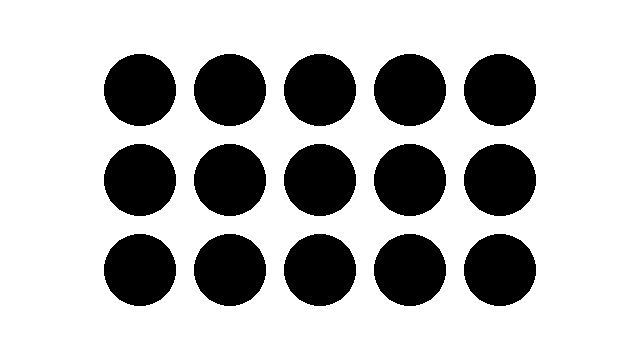
\includegraphics[width=5cm]{images/iter01.png}
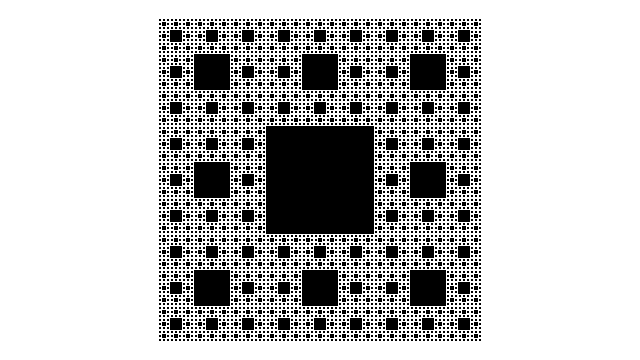
\includegraphics[width=5cm]{images/sier4.png}
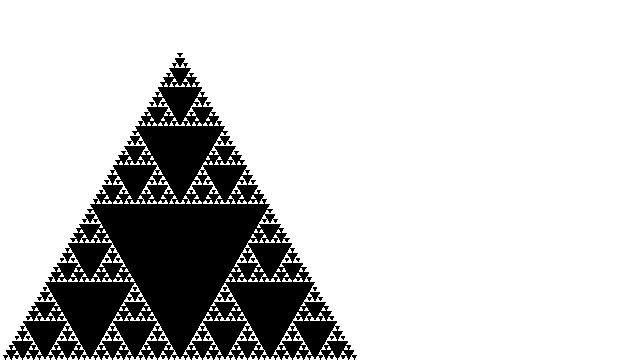
\includegraphics[width=5cm]{images/sier3.png}



\section{Előjeles távolság függvények a síkon}

\subsection{Alapok}

\begin{tcolorbox}[title=Előjeles távolság függvény (signed distance function)]
  Az \emph{előjeles távolság függvény} egy $(x,y)$ pont előjeles távolságát adha meg egy ponthalmaz határától mérve.
  Az egyszerűség kedvéért feltehetjük, hogy az alakzat egy zárt, folytonos, nem önmetsző görbével van megadva.
  $$ t: \mathbb{R}^2 \mapsto \mathbb{R}$$
  $$ t(x, y) = d$$

  Ha $(x,y)$ rajta van az alakzat határán, akkor $t = 0$. Külső pontokra $t$ a pont és az alakzat távolságát adja meg.
  Belső pontokra $t$ negatív előjellel adja meg a pont és a határgörbe távolságát.
  
  Az előjeles távolság függvények meglepően jól használhatók arra, hogy egy képet vagy animációt felépítsünk egyszerű
  alap-alakzatokból.
  \end{tcolorbox}

\matfeladatok


Adjuk meg a következő alakzatok előjeles távolság függvényét:

\begin{enumerate}
  \item Origó középpontú, $r$ sugarú kör.
  \item Origó középpontú, adott méretű, tengely-párhuzamos téglalap.
  \item Végpontjaival adott szakasz.
  \item (*) Szabályos sokszög.
\end{enumerate}

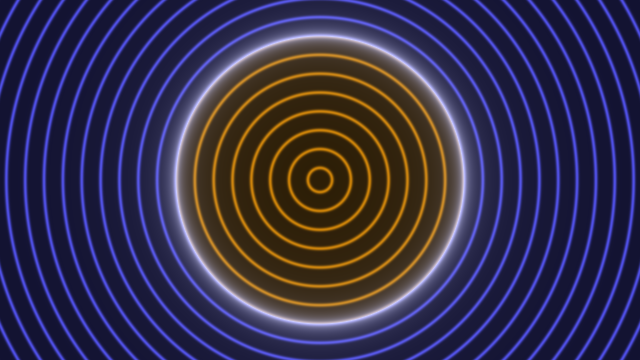
\includegraphics[width=4cm]{images/sdCircle.png}
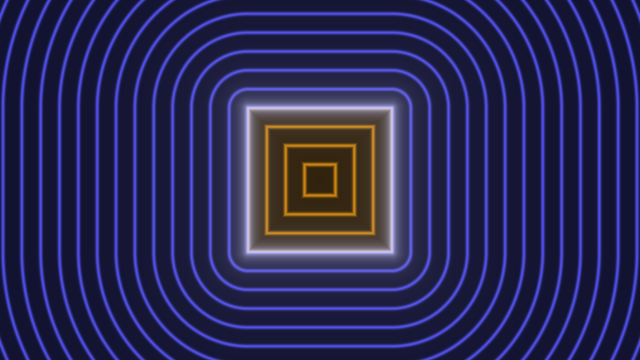
\includegraphics[width=4cm]{images/sdSquare.png}

\includegraphics[width=4cm]{images/sdSegment.png}
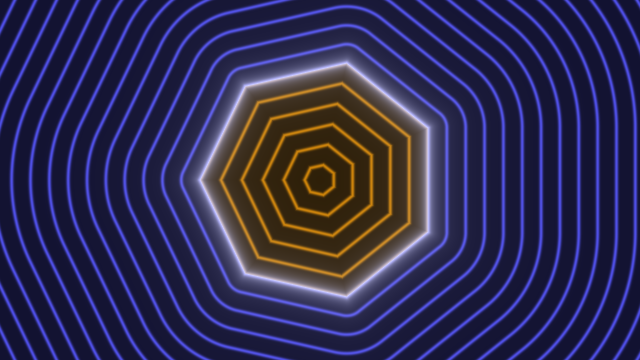
\includegraphics[width=4cm]{images/sdNgon.png}


\subsection{Kompozíció és deformáció}

\matfeladatok

\begin{enumerate}

\item Hogyan írható fel két távolságfüggvénnyel definiált alakzat
(a) uniójának,
(b) metszetének,
(c) különbségének távolságfüggvénye?

\item Hogyan kerekíthető le egy alakzat?

\item Hogyan adható meg egy alakzat (valamilyen vastag) peremének távolságfüggvénye?
\end{enumerate}


\section{Előjeles távolság függvények a térben}

\subsection{Sugár séta algoritmus (ray marching)}

\subsection{Phong megvilágítási modell}

\subsection{Kamera animáció}


\end{document}
